\documentclass{standalone}
\usepackage[dvipsnames]{xcolor}
\usepackage{tikz}
\usetikzlibrary{backgrounds}
\usepackage{contour}
\contourlength{0.66pt}
\usepackage{fontspec}
\setmainfont[Scale=3.0]{Tex Gyre Chorus}

\definecolor{eaglered}{HTML}{A52A2A}
\definecolor{kidagold}{HTML}{FFD700}
\definecolor{hydrapurple}{HTML}{800080}
\definecolor{wolfblue}{HTML}{0038A8}

\tikzset{castle/.pic={
\node () at (0,0) {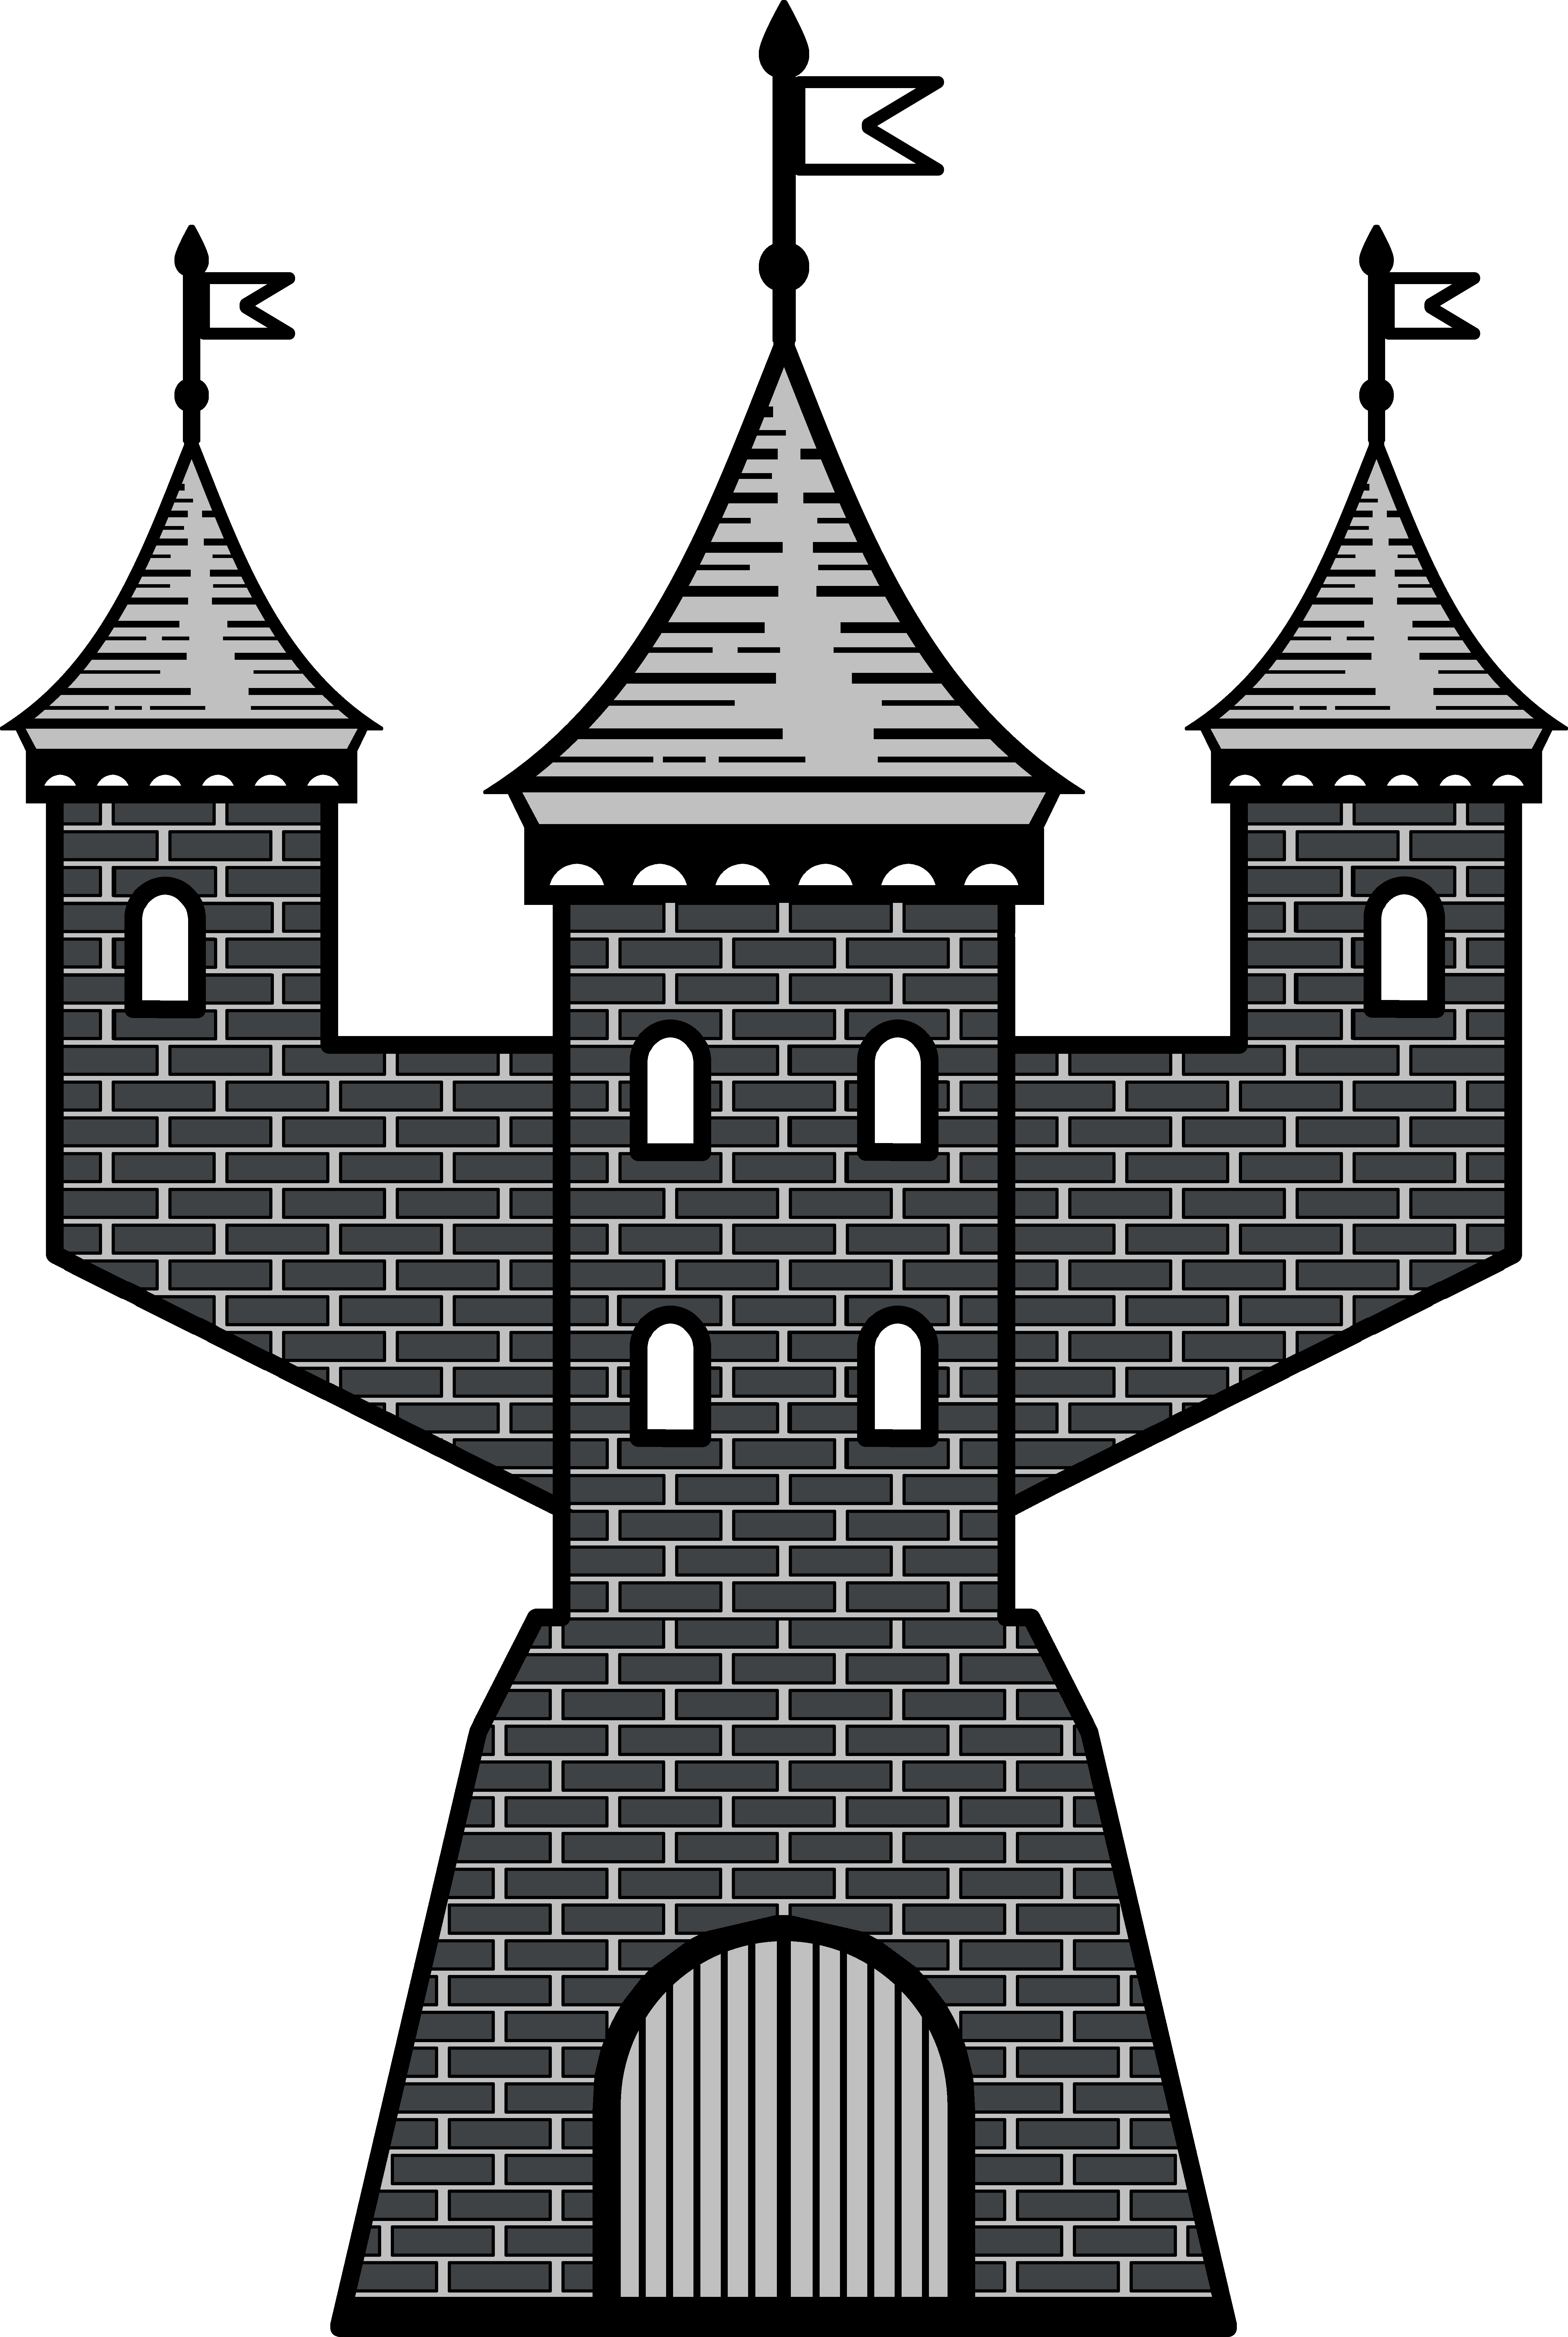
\includegraphics[scale=2.5]{Images/castle.png}};
}}

\tikzset{wolf/.pic={
\node () at (0,0) {
\includegraphics[scale=1.33]{Images/wolf_gray.png}};
}}

\tikzset{eagle/.pic={
\node () at (0,0) {
\includegraphics[scale=1.33]{Images/eagle_brown.png}};
}}

\tikzset{dragon/.pic={
\node () at (0,0) {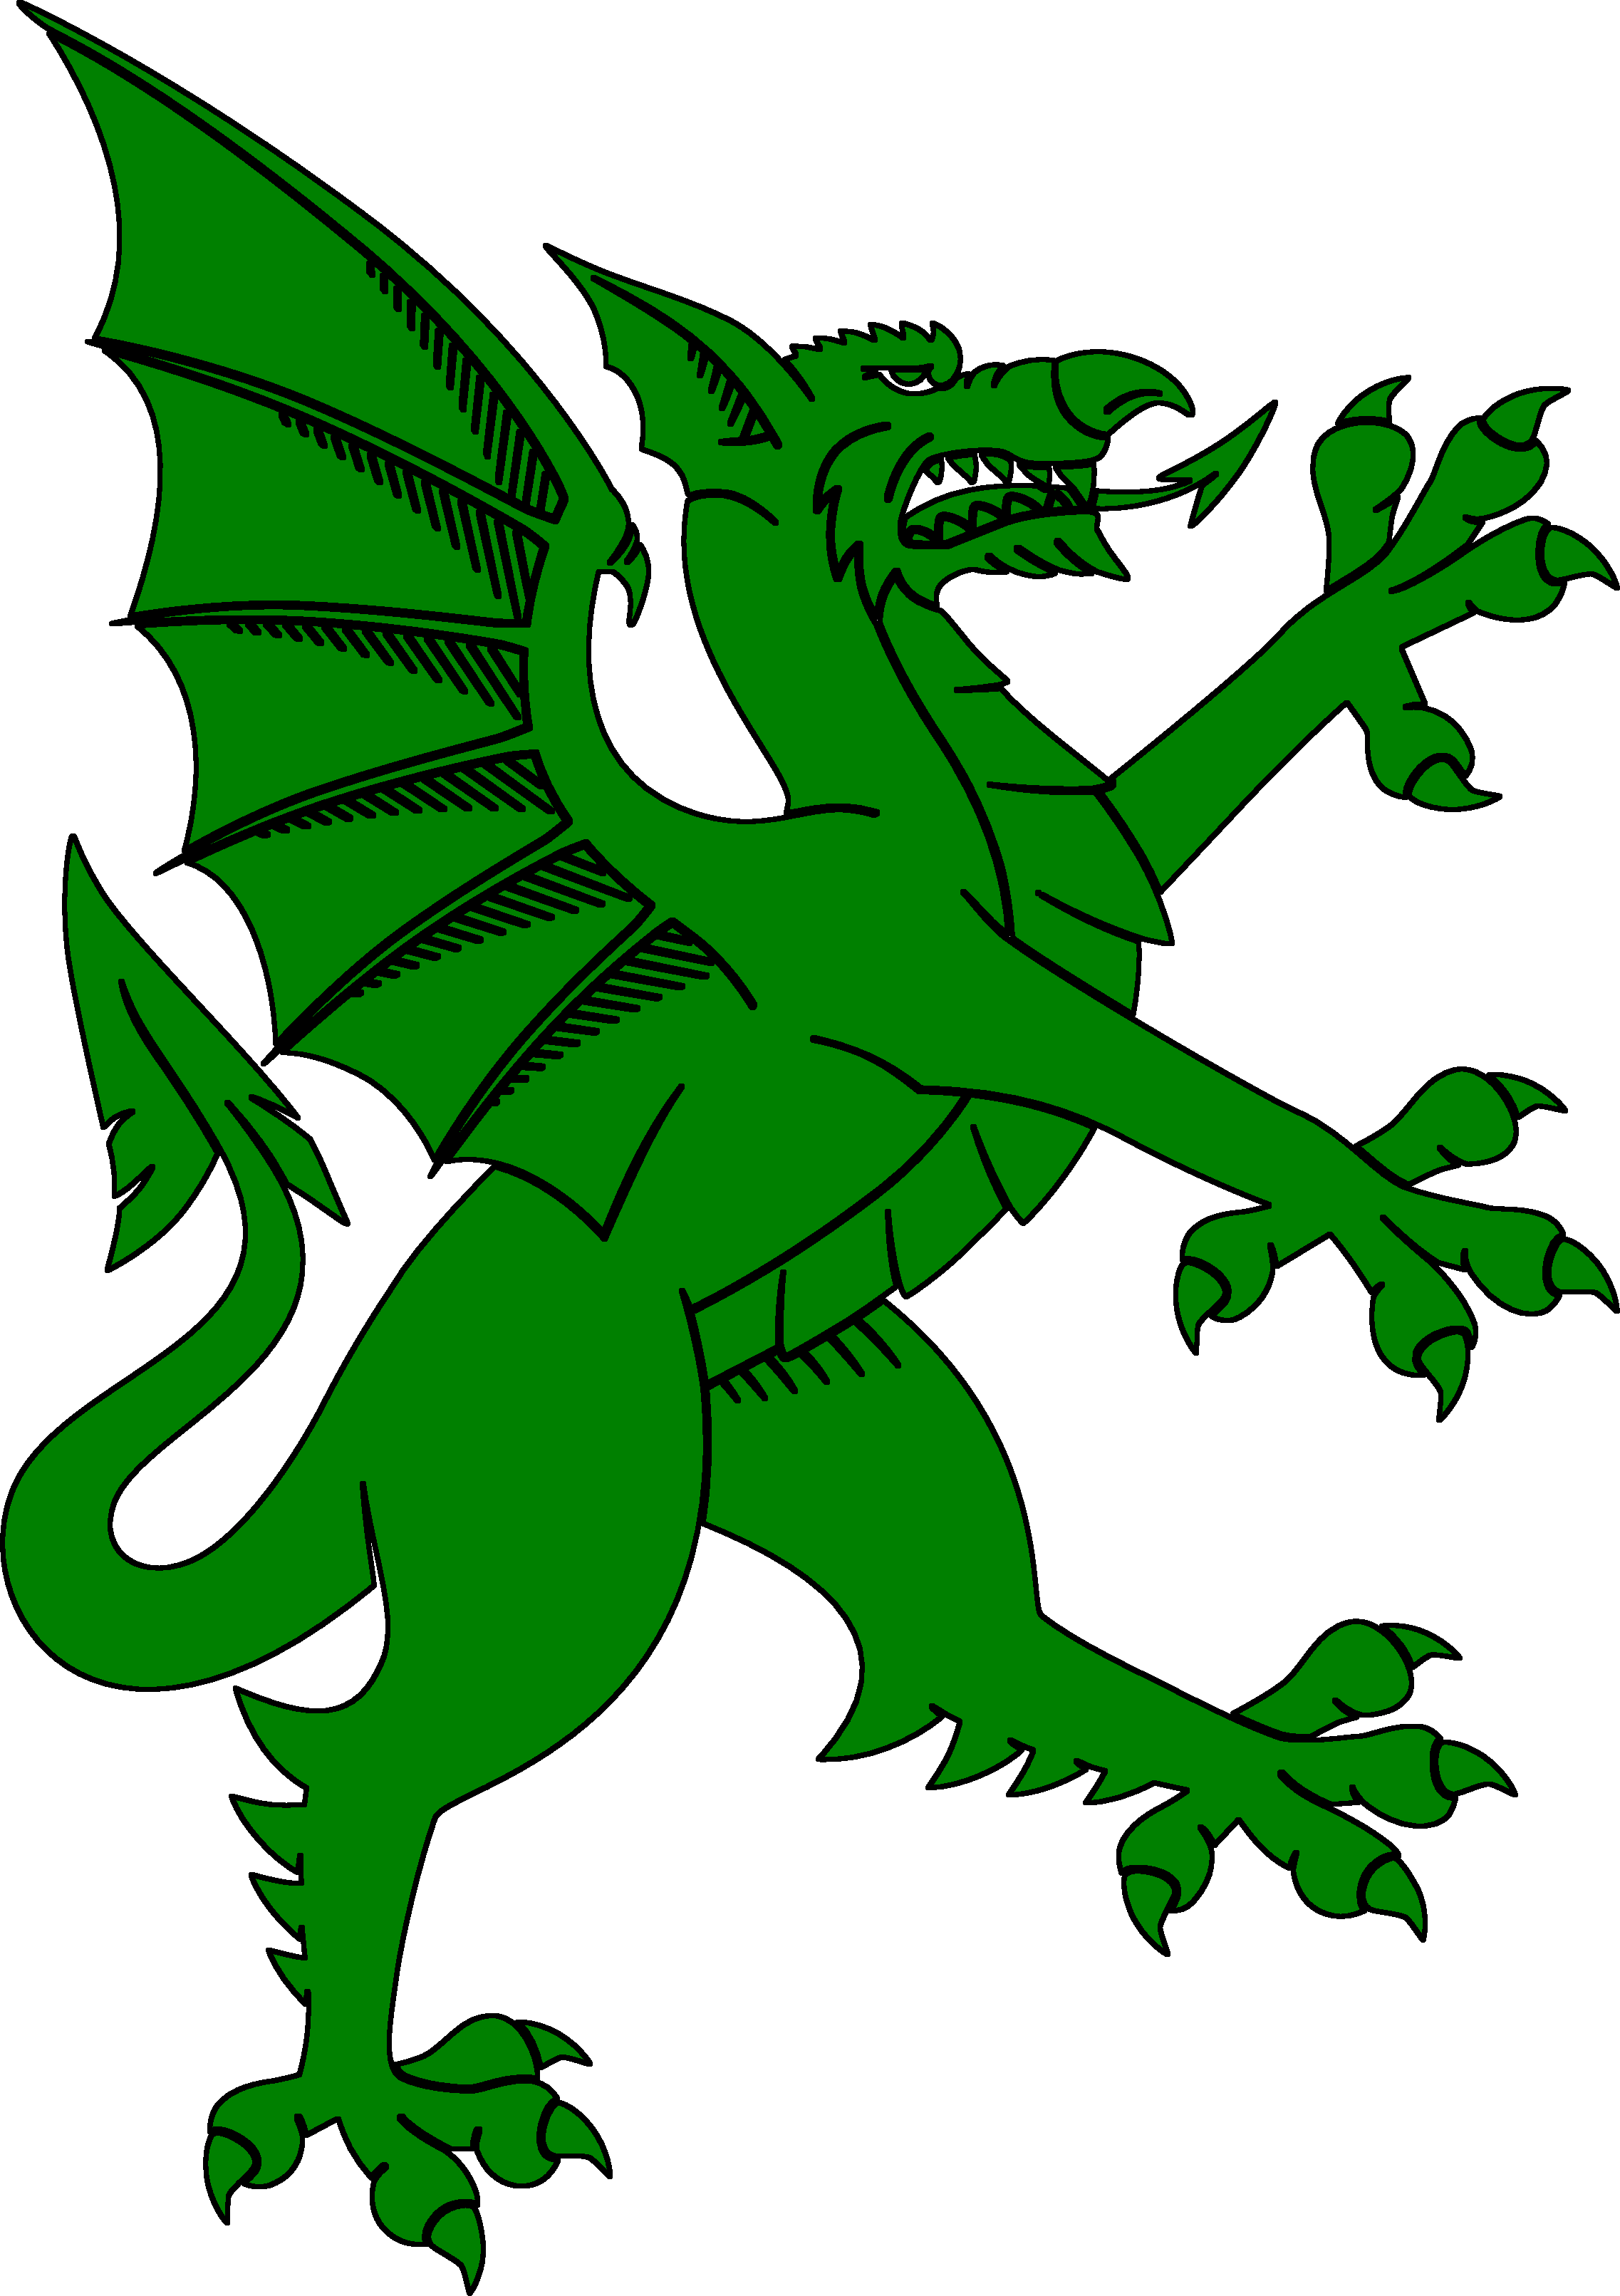
\includegraphics[scale=1.5]{Images/dragon.png}};
}}


\begin{document}
\begin{tikzpicture}[transform shape]
\clip (-5.49,-4.3) -- (-5.49, 4.3) -- (5.69,4.3) -- (5.69,-4.3) -- cycle;
\node at (0,0) {
\includegraphics[scale=0.1]{Images/blue_stone_wall_vector.png}};
\node at (0,2.75) {\contour{black}{\textcolor{WildStrawberry}{\LARGE Castle of Magic}}};
\pic[scale=0.75] at (0.4,-0.375) {eagle};
\pic[scale=0.66, anchor=west] at (2.4,-0.375) {wolf};
\pic[anchor=east, xscale=0.66, yscale=0.66] at (-1.6,-0.125) {dragon};
\node at (0,-3.25) {\contour{black}{\textcolor{WildStrawberry}{\large The Card Game}}};
\end{tikzpicture}
\end{document}